\chapter{Recommended Procedures for Developing Test Cases}
\label{ch:testcaseprocedures}
This chapter presents recommended practices for developing Test Cases.  Some of the material presented is general ``debugging'' practices and useful to other scenarios than just drill string model comparisons; other topics are more specific to the current project, but are items that might be unknown or easily overlooked.  Theses learnings from developing the Test Cases should both help the reader understand why the particular Test Cases were chosen and provide a methodology for developing any new cases.

\section{General Practices}
Drill string models are complex and may be developed in very different manners.  To compare then, it is recommended to use standard best practices for debugging.  These practices are universal regardless if you are debugging a mechanical system or software source code.
\begin{bulletedlist}
	\item Start with the simplest possible case and get that to work first
	\item Vary parameters one by one, changing multiple at a time convolutes behavior and makes it difficult to determine which parameter affected what part of the behavior
    \item Learn the subtle details about how the models work, these often are overlooked and can a significant impact on model behavior
\end{bulletedlist}

\section{Parameters}
Drill string models and contain a number of input parameters.  These parameters are used to make a simulation more realistic, but they are often implemented in different ways in different models.  This makes comparing models challenging.
\begin{numberedlist}
	\item Be mindful of the units, they may be in completely different systems or have subtle definition differences that must be accounted for
	\item Eliminate as many variables as possible by carefully selecting your Test Case
	\item Add parameters back one by one once you have succeeded in matching model behavior
\end{numberedlist}

\section{Practices for Drill String Models}
Below are some practices that are specific to drill string models that can assist in model comparisons.

\begin{definition}{Remove the top drive}
Top drive models can have a dramatic impact on model behavior and they can be a challenge to match.  The tuning parameters used in the model may not translate well to another model.  It is best to start by removing the top drive and matching model behavior.  Once that is done, the top drives can be added back and it is known that any differences are caused by the top drive model.
\end{definition}

\begin{definition}{Start with a vertical borehole}
This removes the effects of the friction model, gravity, and other effects.
\end{definition}

\begin{definition}{Start by removing the tool joints}
This eliminates multiple variables such as how the tool joint stiffness and contact are calculated.
\end{definition}

\begin{definition}{Note how tool joints are handled}
Are the tool joints ignored or directly handled by the model?  If the model does not handle the tool joints internally, it may be necessary to use techniques such as modifying the stiffness (equivalent stiffness) to be able to compare one drill string model to another.  It will also be important to account for the contact and friction in this case.
\end{definition}

\section{Friction Models}
When working with various friction models, it becomes vital to identify parameters that result in similar frictional behaviors.  The parameters for the friction models are static coefficient of friction, dynamic coefficient of friction, and critical velocity. Generally, the static and dynamic coefficients of friction can be equated across different models, while special attention is required to align the critical velocity with the desired frictional behavior.

\subsection{Units}
In the context of modeling torsional dynamics, if the critical velocities of two different models are provided in different units such as meters per second ($m/s$) and revolutions per minute ($RPM$), unit compatibility must first be established for a meaningful comparison. Converting $m/s$ to $RPM$ can be achieved by using
\begin{equation}\label{velocity_conversion}
    V = v\frac{60}{2\pi}r_o
\end{equation}
where $V$ and $v$ are angular velocity expressed in $RPM$, and $m/s$, respectively, and $r_o$ is outer radius of the drill pipe.  Note that this conversion relies on the pipe diameter and thus will, in general, vary along the length of the drill string.  For this reason, it is preferred that the input units for the critical velocity to be linear and the conversion be done internally by the drill string model on each pipe segment.

% \wordingstart{} After matching the units, the critical angular velocity of the model, which is for the comparison, can be decided by comparing the frictional force with respect to angular velocity. \wordingend{}
%For instance, considering Test Case 2 with a critical velocity of 0.03 $m/s$ and a drill string radius of 0.075 $m$, the critical velocity can be converted to 4$RPM$.

\section{Coulomb versus Stribeck Friction Models}
Coulomb and Stribeck friction models both account for sliding friction.  The Coulomb model is simpler and is a step function that alternates from the static friction coefficient and dynamic friction coefficient.  The critical velocity may take any, but is frequently assume to be zero.  The Stribeck model is a little more sophisticated and assumes an exponential decay between the static and dynamic coefficients of friction.  In the more general cases, both models may assume an increase in the friction coefficient as the velocity increases (this effect is not included for this project).

To compare a model that uses a Coulomb friction model to one that uses a Stribeck model, the challenge is in selecting the appropriate critical velocity.  To demonstrate this, \figurename~\ref{figure:stribeck_coulomb_friction} shows an example comparison between Coulomb and Stribeck friction models. It compares two different critical velocities of a Coulomb model with a Stribeck model.
\begin{figure}
	\centering
	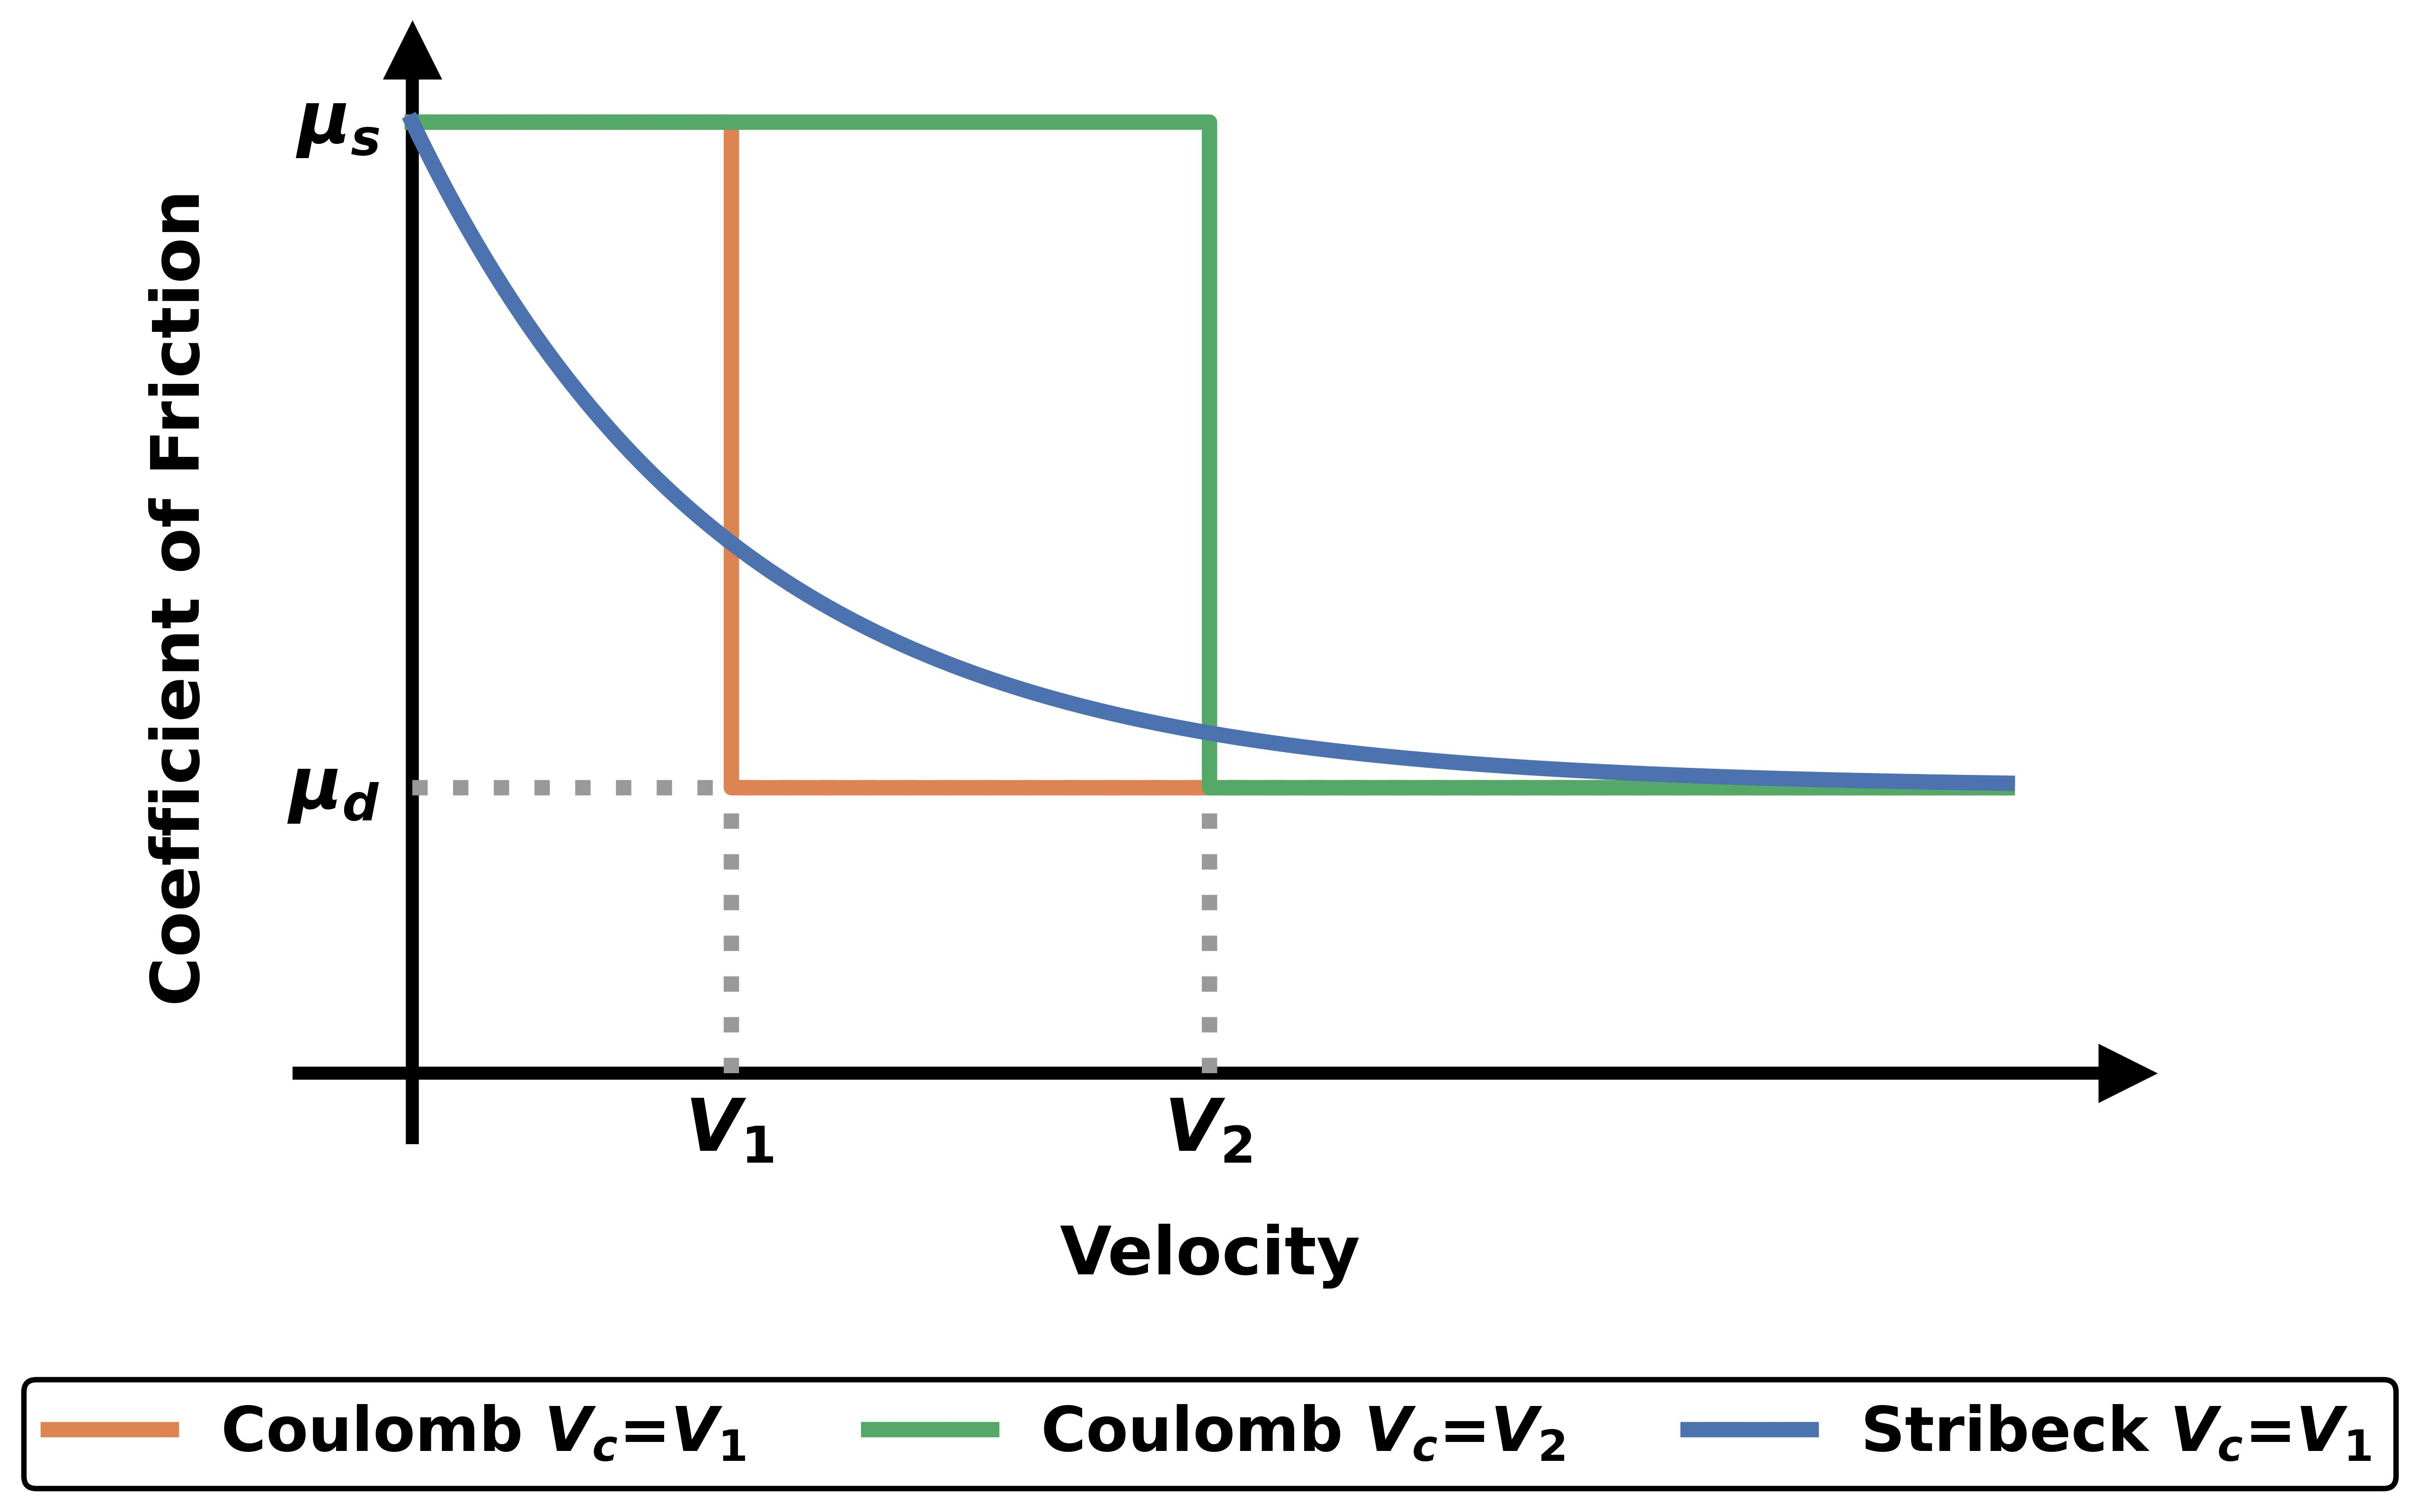
\includegraphics[height=2.25in]{Stribeck_Coulomb_friction}
    \caption[Comparison between Coulomb and Stribeck friction model]{A comparison between Coulomb and Stribeck friction models. A Stribeck model with a critical velocity of $V_1$ is compared to Coulomb friction models with critical velocities of $V_1$ and $V_2$. $\mu_s$ and $\mu_d$ indicate the static and dynamic coefficients of friction, respectively, and $V$ is the velocity.  The Coulomb model with a critical velocity of $V_1$ matches the critical velocity of the Stribeck friction.  The choice of $V_2$ as the critical velocity for the Coulomb friction is closer to the point where the Stribeck model coefficient begins to significantly increase.}
	\label{figure:stribeck_coulomb_friction}
\end{figure}
The Coulomb model with a critical velocity of $V_1$ matches the critical velocity of the Stribeck friction.  The choice of $V_2$ as the critical velocity for the second Coulomb friction curves moves the change from static to dynamic coefficients of friction to the point where the Stribeck model coefficient begins to significantly increase.

There are arguments for selecting either $V_1$ or $V_2$.  The choice $V_1$ seems to be a natural choice.  It is the same value the Stribeck model uses as its critical velocity.  In addition, as a method to measure how close the curves are, we could calculate the area under the curves.  In \figurename~\ref{fig:frictionmodelareaundercurves}, this is demonstrated.
\begin{figure}
	\begin{minipage}[t]{\linewidth}
		\begin{minipage}[t]{0.325\linewidth}
			\centering
			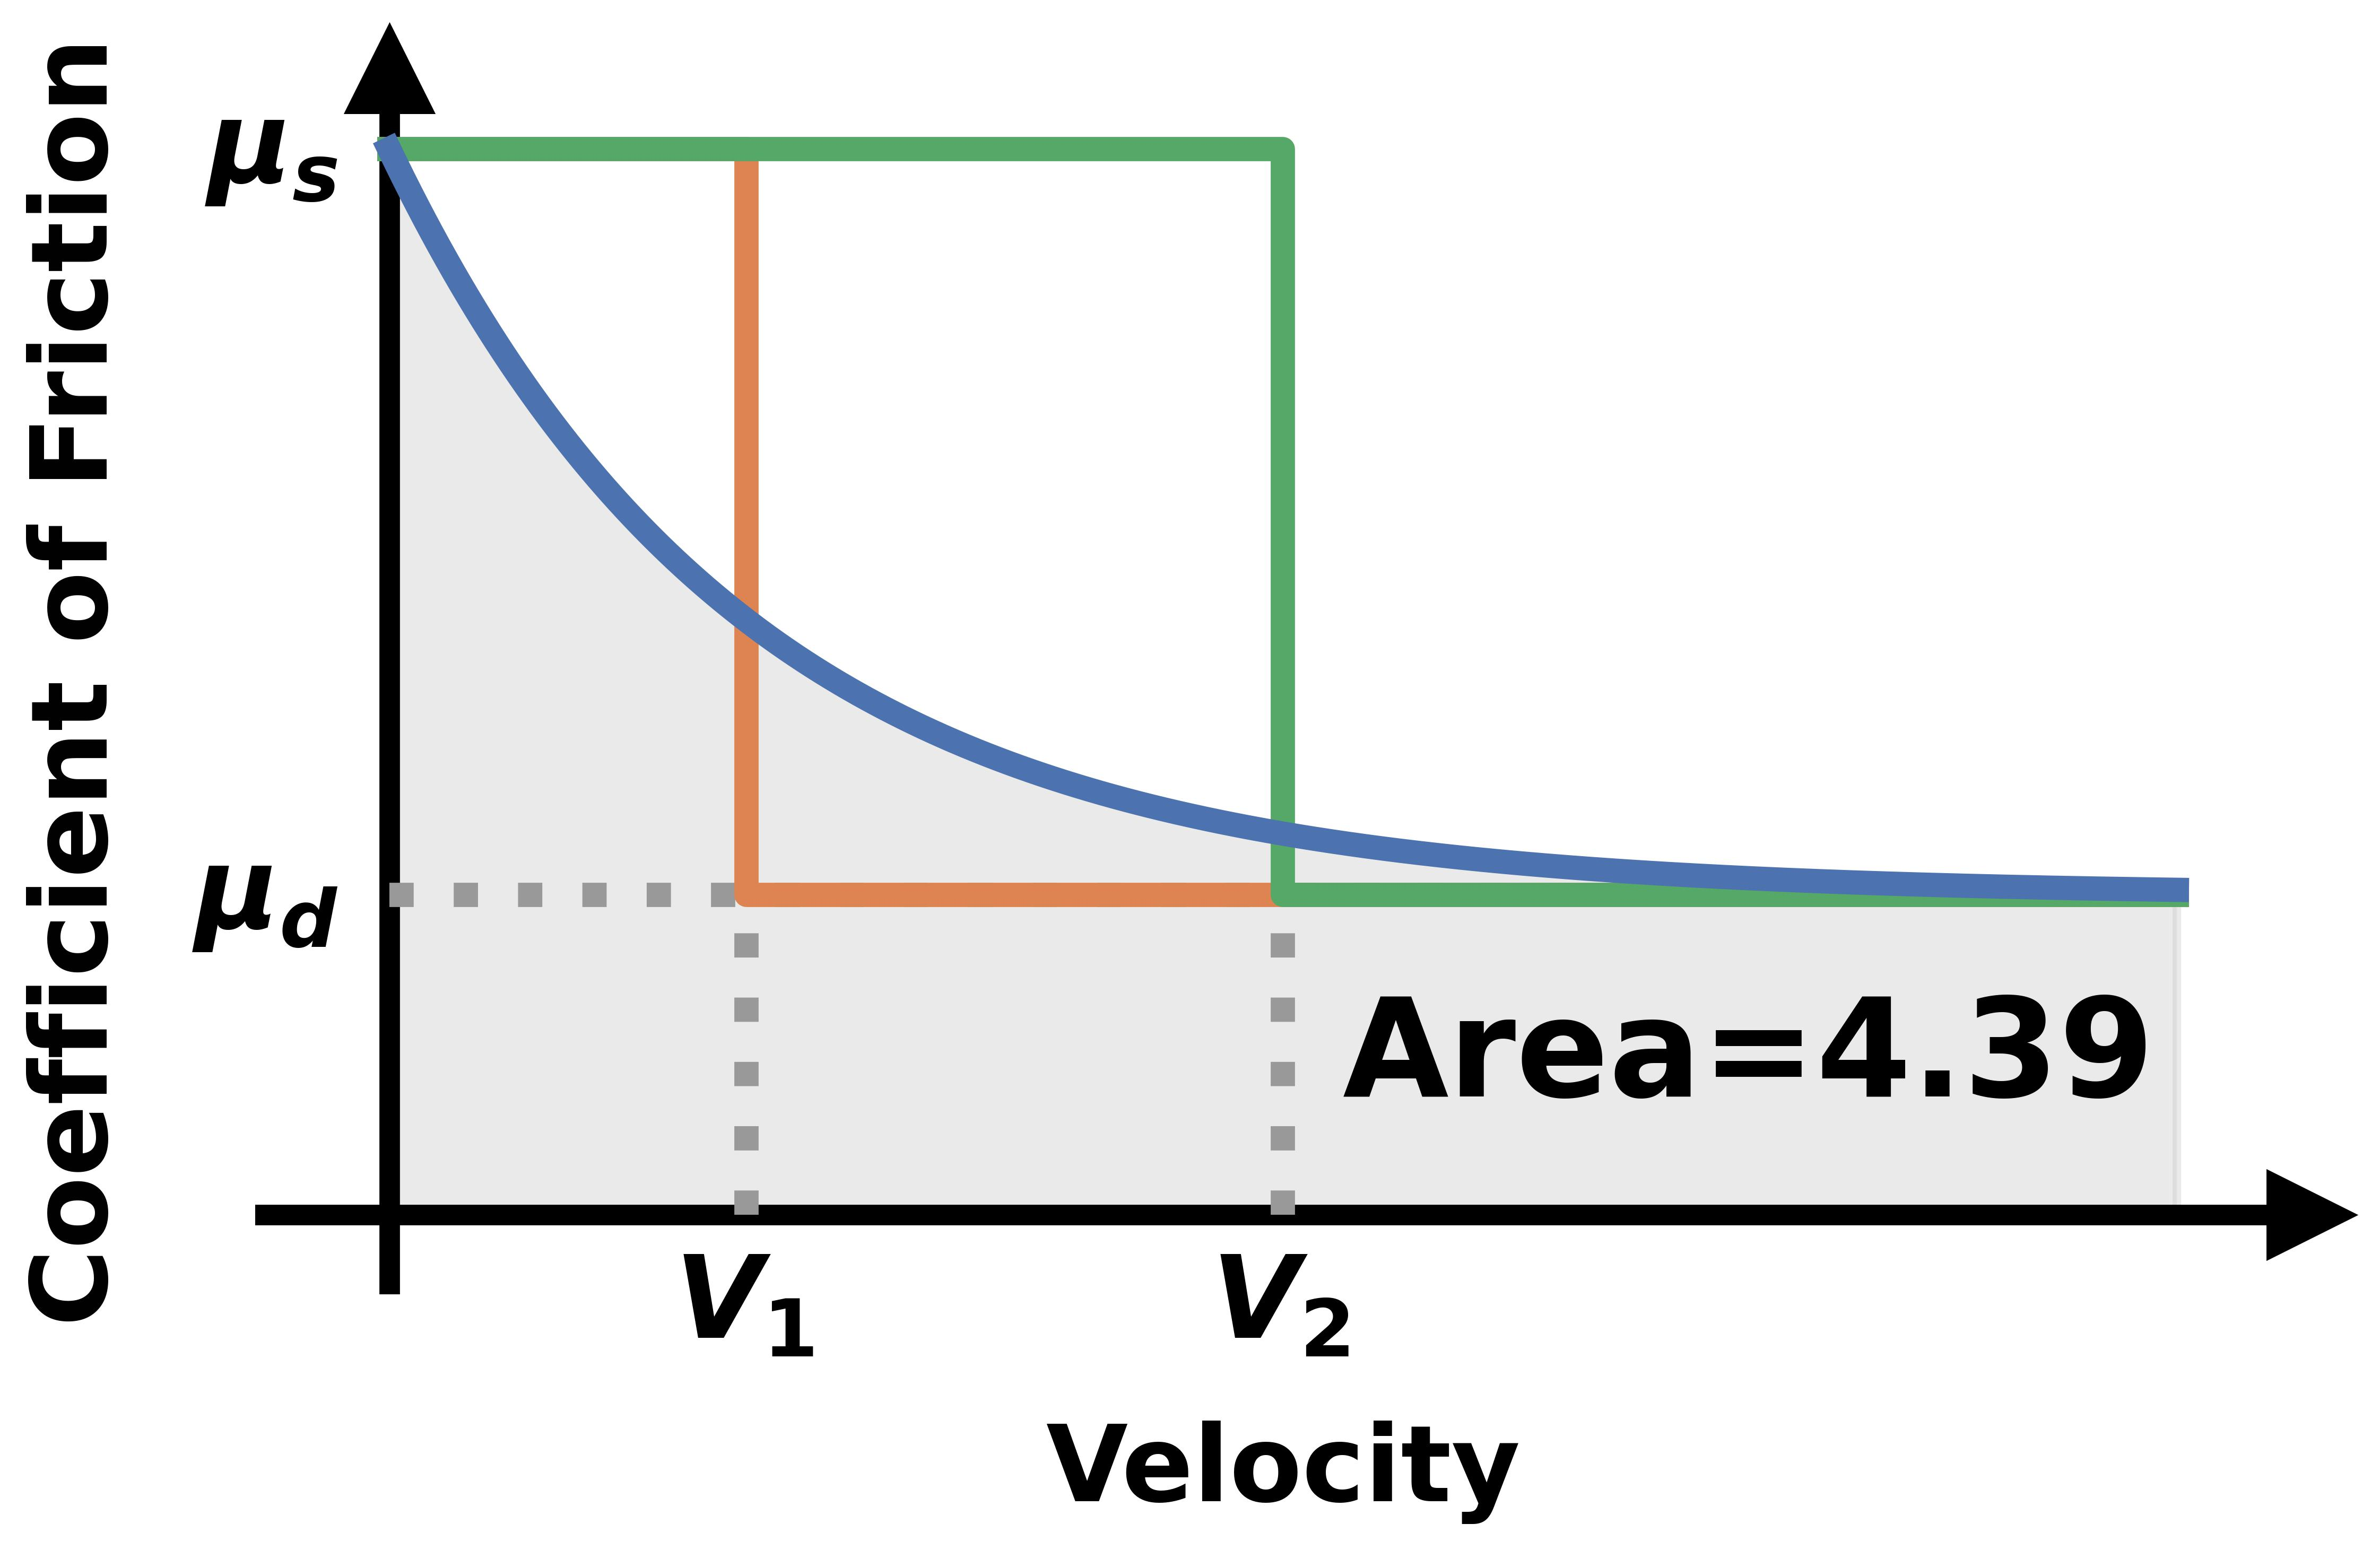
\includegraphics[width=\linewidth]{Stribeck_Coulomb_friction_filled_2}
			\subcaption{Stribeck friction curve with a critical velocity of $V_1$.}
			\label{fig:Stribeck_Coulomb_friction_filled_2}
		\end{minipage}
		\hfill
		\begin{minipage}[t]{0.325\linewidth}
			\centering
			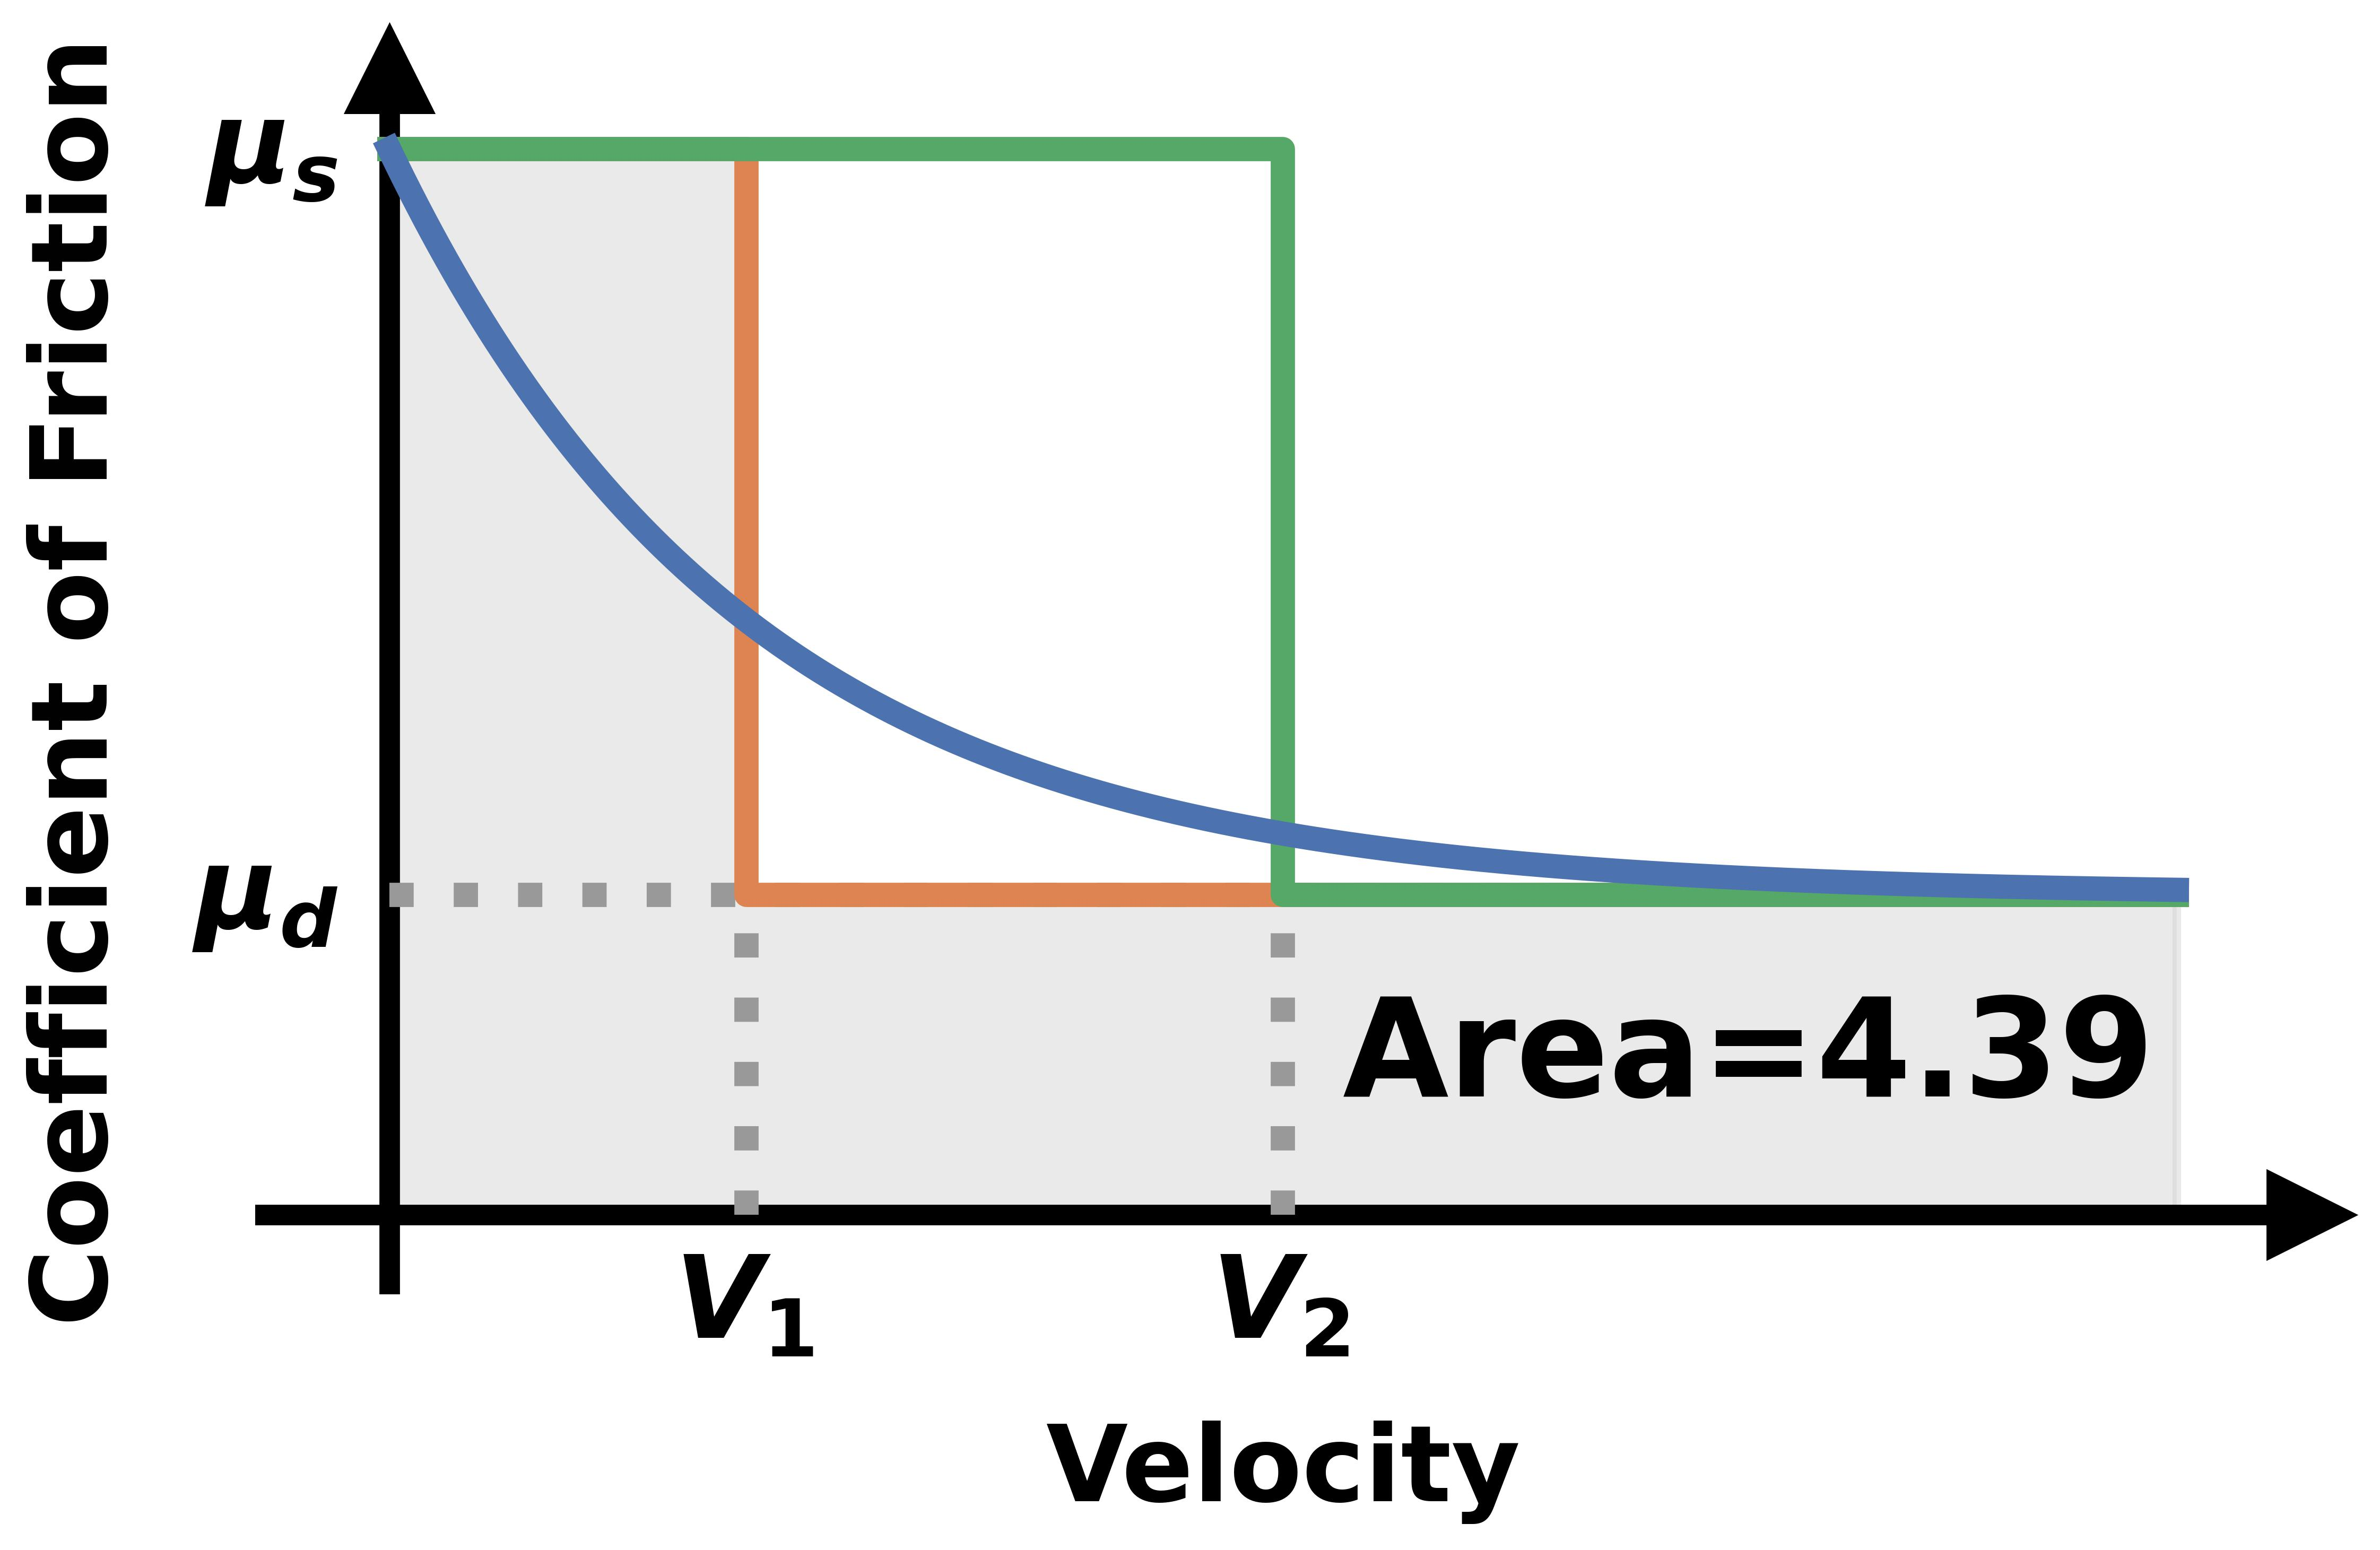
\includegraphics[width=\linewidth]{Stribeck_Coulomb_friction_filled_0}
			\subcaption{Coulomb friction curve with a critical velocity of $V_1$.}
			\label{fig:Stribeck_Coulomb_friction_filled_0}
		\end{minipage}
		\hfill
		\begin{minipage}[t]{0.325\linewidth}
			\centering
			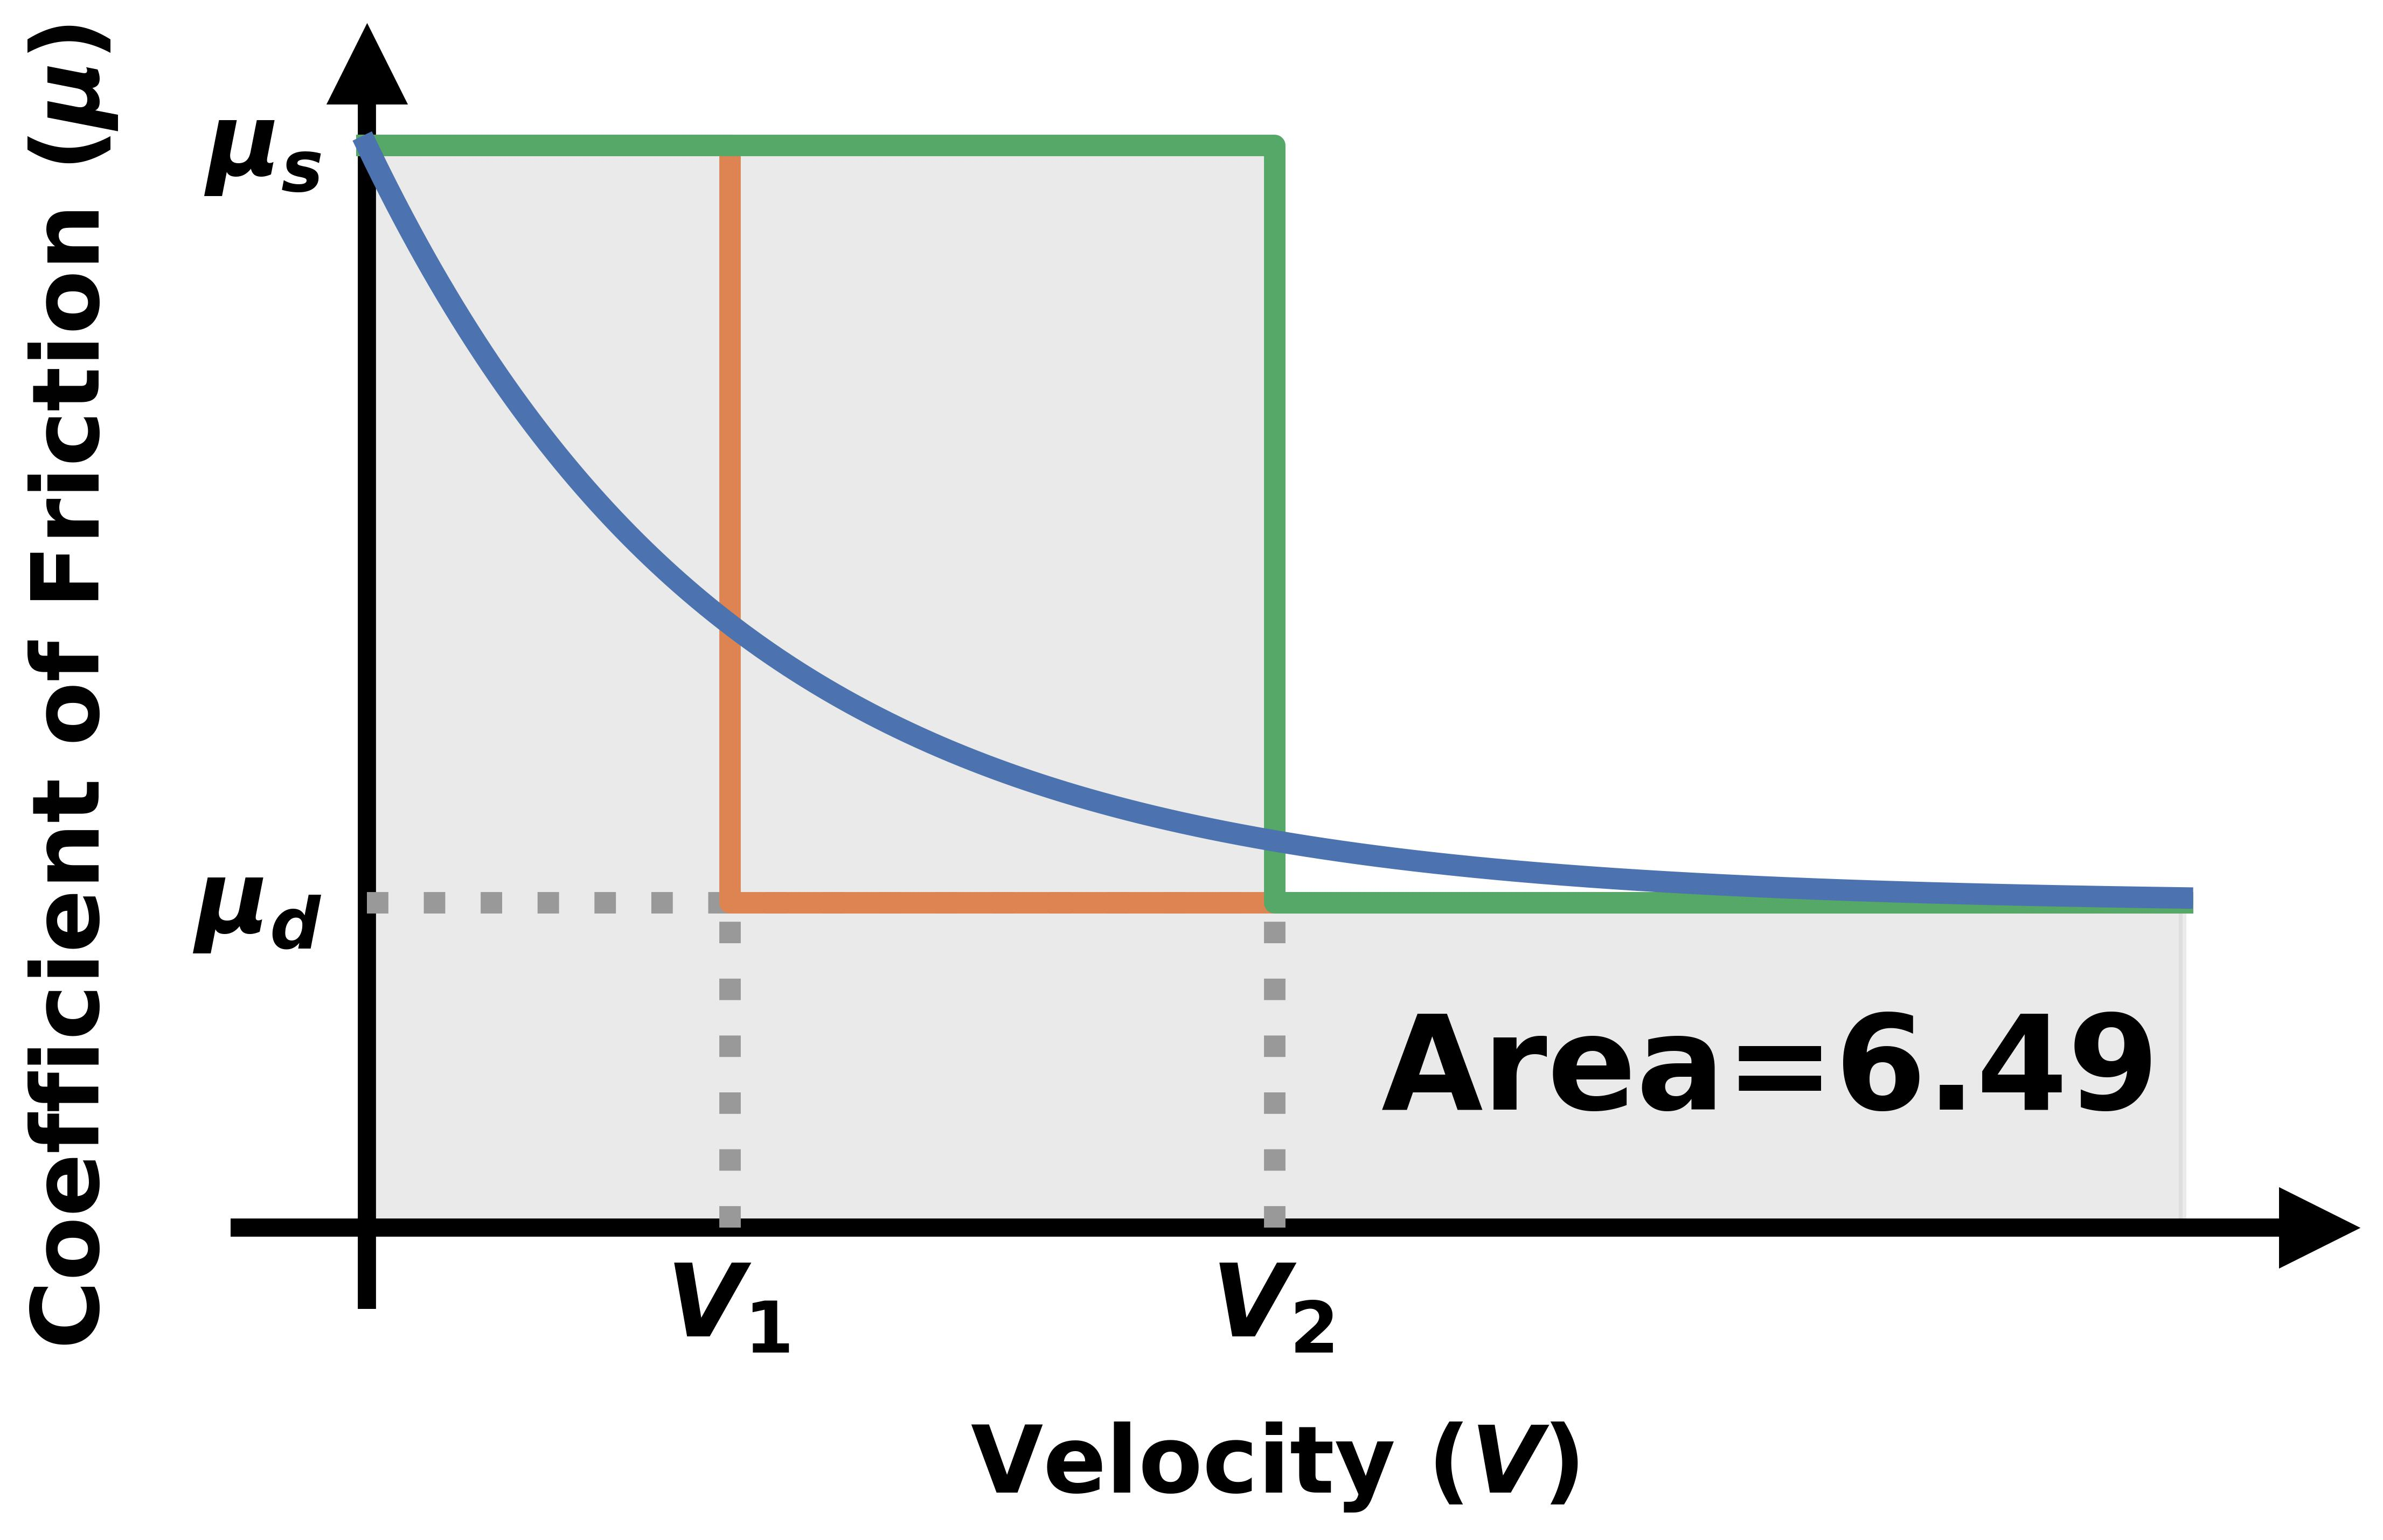
\includegraphics[width=\linewidth]{Stribeck_Coulomb_friction_filled_1}
			\subcaption{Coulomb friction curve with a critical velocity of $V_2$.}
			\label{fig:Stribeck_Coulomb_friction_filled_1}
		\end{minipage}
	\end{minipage}
    \caption[Areas under friction curves]{The areas under the friction curves are used as a measurement of how close the curves are to each other.  The choice of $V_1$ for the critical velocity of the Coulomb friction in~(\subref{fig:Stribeck_Coulomb_friction_filled_0}) creates an area under the curve which is closer to the Stribeck curve shown in~(\subref{fig:Stribeck_Coulomb_friction_filled_2}).  The choice of $V_2$ for the critical velocity of the Coulomb model, shown in in~(\subref{fig:Stribeck_Coulomb_friction_filled_1}), leads to a larger area.  The areas were calculated for the velocity range of $[0, 2V_2]$.  The legend from \figurename~\ref{figure:stribeck_coulomb_friction} is applicable here as well.}
	\label{fig:frictionmodelareaundercurves}
\end{figure}
It can be seen that, on average, the coefficient of friction from the Coulomb model with a critical velocity of $V_1$ is a close match to the Stribeck model.  The argument for selection $V_2$ is that it is closer to when the Stribeck model coefficient of friction begins to increase and this may better match the behavior of the Stribeck model.  It should be noted, these are only two choices and others are possible as well.  The choice of what critical velocity to use is non-obvious.  Therefore, testing should be conducted to determine the best value.

Some preliminary testing indicated $V_2$ gave a better match between models\footnote{The results are not included as part of this report.}.  Therefore, in this project, we selected a critical angular velocity that corresponds to $V_2$ for the Coulomb model. This choice allows us to align the exponentially decreasing component of the Stribeck model with the end point of static friction of the Coulomb friction model.  However, it should be noted that this may not be a universal selection and further testing should be performed to investigate further.

%However, it is important to note that additional tests involving different angular velocities have been performed and are included in the appendix chapter for comprehensive analysis. 